\documentclass[border=2pt]{standalone}
\usepackage{tikz}
\usetikzlibrary{quotes,angles}
\usepackage{amsmath}

\begin{document}

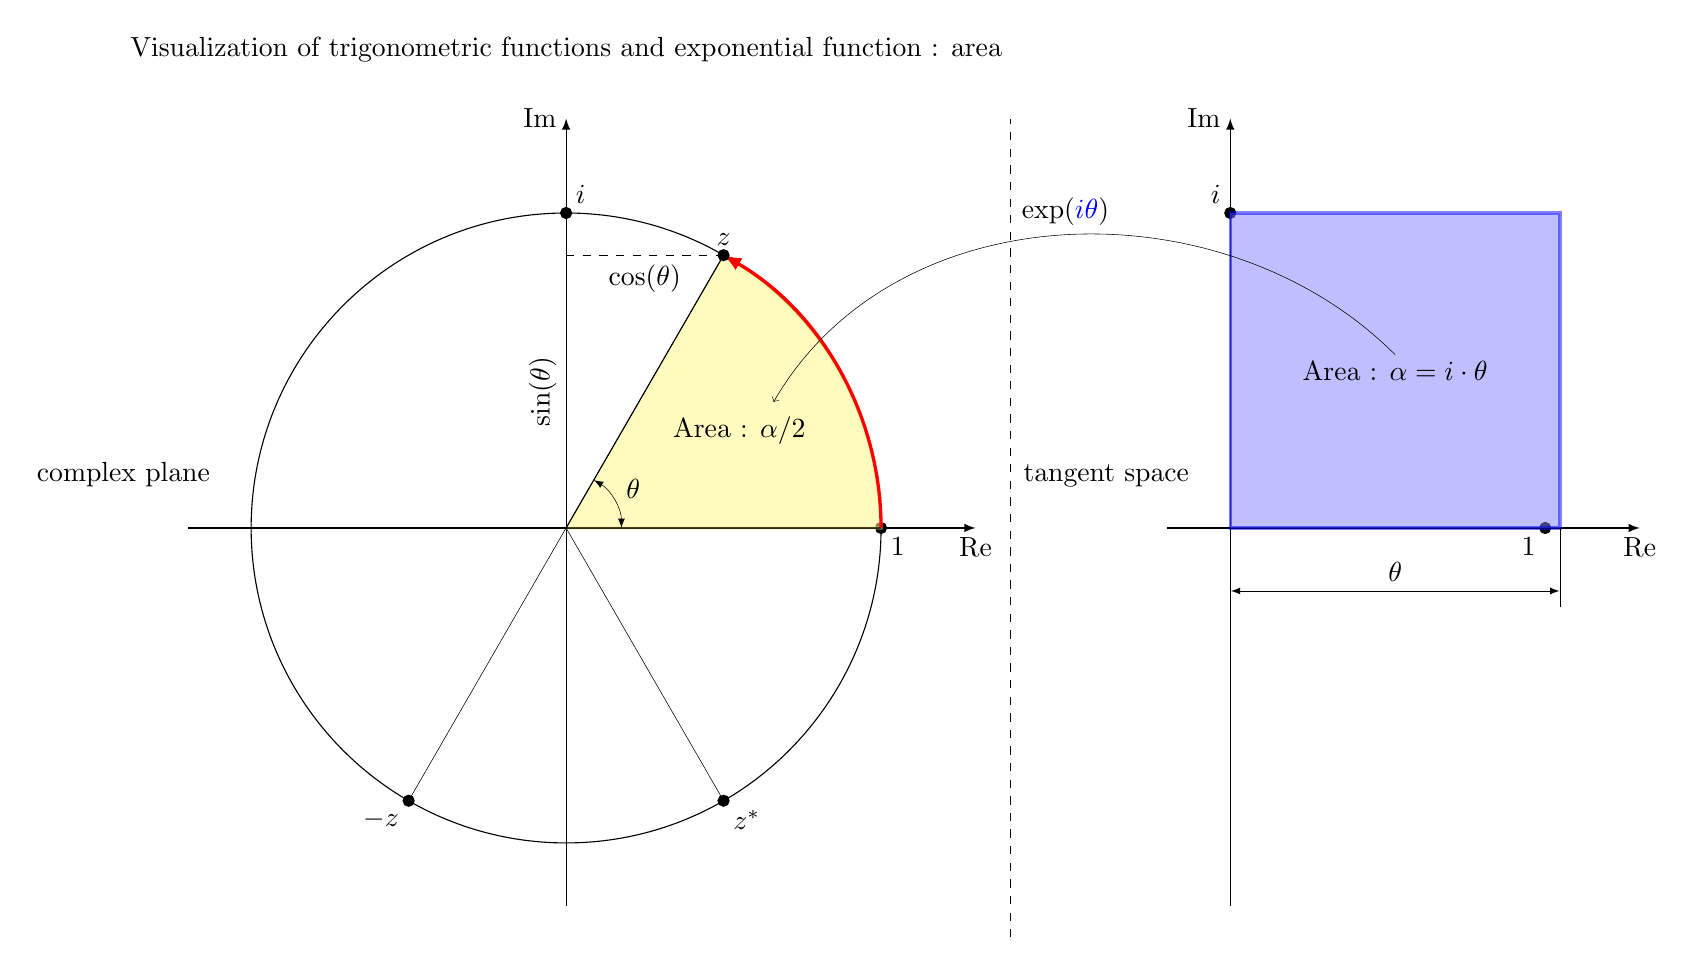
\begin{tikzpicture}[scale=4]

% Draw x and y axis lines
\draw [->,>=latex] (-1.2,0) -- (1.30,0) node [below] {$\mathrm{Re}$};
\draw [->,>=latex] (0,-1.2) -- (0,1.30) node [left ] {$\mathrm{Im}$};
\node[above left] at (-1.1, 0.1) {complex plane};
\filldraw[black] (1,0) circle (0.5pt) node[below right] {$1$} ;
\filldraw[black] (0,1) circle (0.5pt) node[above right] {$i$} ;
\node[above] at (0.0,1.45) {Visualization of trigonometric functions and exponential function : area};

% Draw a circle at the origin of radius 1
\draw (0,0) circle (1);

\pgfmathsetmacro{\angle}{60}
\pgfmathsetmacro{\length}{\angle / 180 * pi}

% Draw a yellow arc at the origin of radius 1
\filldraw[very thick,draw=yellow!50,fill=yellow!50,opacity=0.5]
(0,0) -- (00:1) arc (00:\angle:1) ;

\draw [->,>=latex, very thick, red] (1,0) arc (0:\angle:1) ;

\draw
  (1,0) coordinate (a) 
  -- (0,0) coordinate (b) 
  -- ( {cos(\angle)}, {sin(\angle)} ) coordinate (c) 
  pic["$\theta$", draw=black, very thin, <->,>=latex, angle eccentricity=1.4, angle radius=20]
  {angle=a--b--c};


\draw [very thin, dashed] ( 0, 0) -- node[above, rotate=90] {$\sin(\theta)$} ( 0, {sin(\angle)}) ;
\draw [very thin, dashed] ( 0, {sin(\angle)}) -- node[below] {$\cos(\theta)$} ( {cos(\angle)}, {sin(\angle)}) ;

\draw [very thin] (0,0) -- ( {cos(\angle)}, {sin(\angle)}) ;
\draw [very thin] (0,0) -- ( {cos(\angle)},-{sin(\angle)}) ;
\filldraw[black] ( {cos(\angle)}, {sin(\angle)}) circle (0.5pt) node[above] {$z$} ;
\filldraw[black] ( {cos(\angle)},-{sin(\angle)}) circle (0.5pt) node[below right] {$z^*$} ;
\draw [very thin] (0,0) -- (-{cos(\angle)},-{sin(\angle)}) ;
\filldraw[black] (-{cos(\angle)},-{sin(\angle)}) circle (0.5pt) node[below left] {$-z$} ;

% Draw a string at center.
\node[below] at ({cos(\angle)+0.05}, {sin(\angle)/2-0.05}) {Area : $\alpha/2$};



\begin{scope}[xshift=60]

\draw [very thin, dashed] (-0.7,-1.3) -- (-0.7, 1.30) ;
\draw [->,>=latex] (-0.2,0) -- (1.30,0) node [below] {$\mathrm{Re}$};
\draw [->,>=latex] (0,-1.2) -- (0,1.30) node [left ] {$\mathrm{Im}$};
\node[above left] at (-0.1, 0.1) {tangent space};
\filldraw[black] (1,0) circle (0.5pt) node[below left] {$1$} ;
\filldraw[black] (0,1) circle (0.5pt) node[above left] {$i$} ;

\filldraw[very thick,draw=blue,fill=blue!50,opacity=0.5] (0,0) rectangle (\length, 1);
\draw [very thin] (\length, 0.0) -- (\length, -0.25);
\draw [very thin, |<->|,>=latex] ( 0.0, -0.2) -- node[above] {$\theta$} (\length, -0.2);

\node at (\length/2, 1/2) {Area : $\alpha = i \cdot \theta$};

\draw [very thin, ->] (\length/2, 1/2+0.05) to [out=135,in=60] node[above ] {$\exp(\color{blue}i\theta\color{black})$}  (-1.45, 0.40);

\end{scope}


\end{tikzpicture}

\end{document}

